\documentclass[main.tex]{subfiles}
\begin{document}
\begin{enumerate}

\subsection*{Section 7}
	
\item Answer the following questions about LANs (wired and wireless):

    \begin{enumerate}
        \item Describe (through some pseudo code and sufficient explanation) CSMA/CD and Binary Exponential Backoff as used in IEEE 802.3 Ethernet.
        \item Describe CSMA/CA (through some pseudo code and sufficient explanation) as used in IEEE 802.11 WiFi.
    \end{enumerate}
    
\item M terminals are attached by a dedicated pair of lines to a hub in a star topology (Figure \ref{fig:20q_a}). The distance from each terminal to the hub is d meters, the speed of the transmission lines is R bits/second, all frames are f length 12,500 Bytes, and the signal propagates on the line at speed of $2.5^{*} 10^{8}$ meters/second. For M=6 terminals, d=25 meters and R = 10Gbps, what is the maximum network throughput achievable when the hub is implementing slotted ALOHA?

\begin{figure}
\centering\fbox{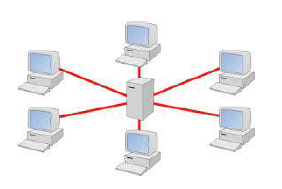
\includegraphics[width=3.0in]{figures/2018s/20q_a.png}}
\caption{Star Topology}
\label{fig:20q_a}
\end{figure}

\item Consider a data link layer with the following parameters: Frame transmission time at the sender is $\mathrm{t}_\mathrm{f}=20$ microseconds. ACK or NAK transmission time at the receiver is $\mathrm{t}_\mathrm{ack} = 10$ microseconds. Link propagation delay on both directions is $\mathrm{t}_{\mathrm{prop}} = 25$ microseconds. Suppose frame processing time at both sender and receiver is negligible, i.e., $\mathrm{t}_{\mathrm{prop}] = 0$. Finally, overall round-trip probability of frame error on the link is $r=0.04$. 

    \begin{enumerate}
        \item Assume that for the Stop-and-wait ARQ scheme, the TIMEOUT at the sender is chosen optimally. What is the resulting throughput (frames/second)?
        \item  In the Go-Back-N ARQ scheme, if the link is error free, what is the minimum window size $N$ that is able to keep the link busy?
        \item Choose window size in Part b and now consider the link error probability $r=0.04$. What the throughput (frames/second) of the Go-Back-N ARQ scheme?
    \end{enumerate}

\end{enumerate}
\end{document}